\subsection{Performance Requirements}
\begin{itemize}
	\item Reliability: The correct algorithms, datasets and experiments should be returned when requested. \newline
    \item Data Integrity: Consistent, correct and complete output should always be generated for all supported input. \newline
\end{itemize}
\subsection{Design Constraints}
\begin{enumerate}
	\item PLEASE FILL IN...
\end{enumerate}
\subsection{Software System Attributes}
\begin{flushleft}
    \par\textbf{Extensibility}: More future features and objects can be added to the input unit seamlessly without affecting the functionality of the code because the client and the underlying structure of the Experiment object have been decoupled. .\newline
    
    \par\textbf{Modifiability: } The Builder design pattern enables the input unit to be highly customizable without affecting the client and other functionalities that depend on it negatively.\newline
  
    \par\textbf{Robustness}: Object modification an side-effect generations are minimized which ensures that few code failures are generated.. \newline
    \end{flushleft}

\subsection{Class diagram}
	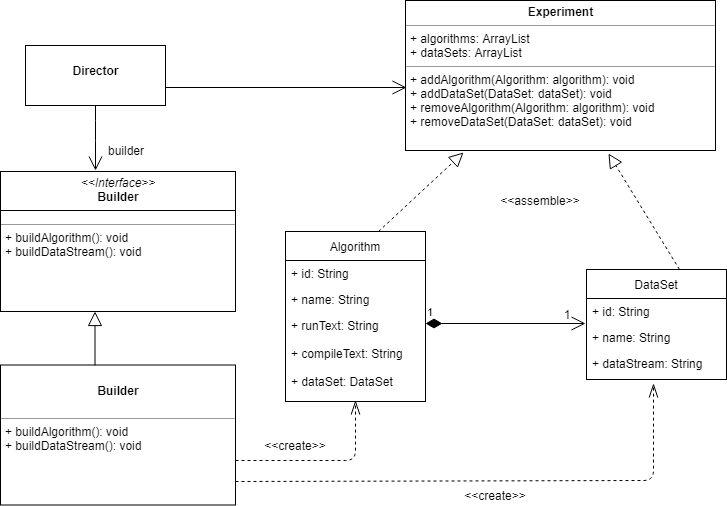
\includegraphics[width=\textwidth]{input_unit/images/input_unit_class_diagram.png}
	\begin{center}
	    \small{Figure 1: Class diagram for Input Unit}
    \end{center}
 \begin{flushleft}
\par\textbf{Design Pattern Used: }
	I used the Builder design pattern because it enables the Algorithm and DataSet objects to be configurable so that multiple types of data sets, compilation environments and executables can be considered with minimal effort to the developer. The consumer of the service has no access to the underlying structure of the object requested and so decoupling is highly utilized.
    \end{flushleft}
	
\subsection{Activity diagrams for Input Unit}
	\subsubsection{Create Algorithm}
    \par With regards to Experiment and Data sets,
{ \textit{Mutatis muntandis} the same as regarding algorithms.} \newline \newline
    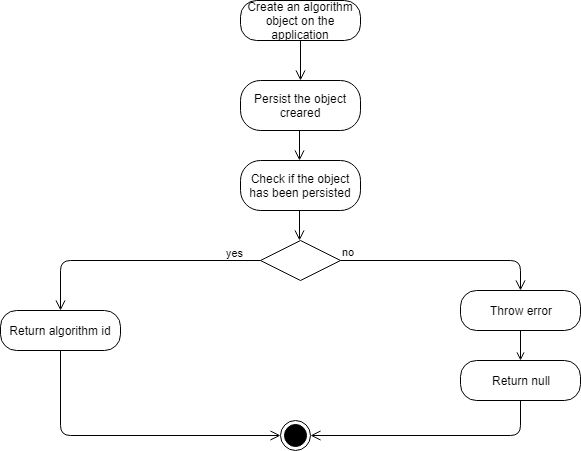
\includegraphics[width=\textwidth]{input_unit/images/create_algorithm_activity_diagram.png}
	\begin{center}
	    \small{Figure 2a: Activity diagram for Creating an algorithm }
    \end{center}
    
    \subsubsection{Remove Algorithm}
    \par With regards to Experiment and Data sets,
{ \textit{Mutatis muntandis} the same as regarding algorithms.} \newline \newline
    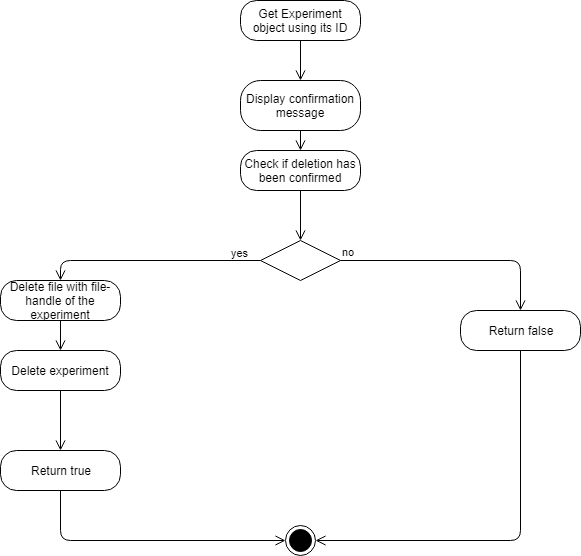
\includegraphics[width=\textwidth]{input_unit/images/delete_activity_diagram.png}
	\begin{center}
	    \small{Figure 2b: Activity diagram for Deleting an algorithm }
    \end{center}
    
    \subsubsection{Get Algorithm}
    \par With regards to Experiment and Data sets,
{ \textit{Mutatis muntandis} the same as regarding algorithms.} \newline \newline
    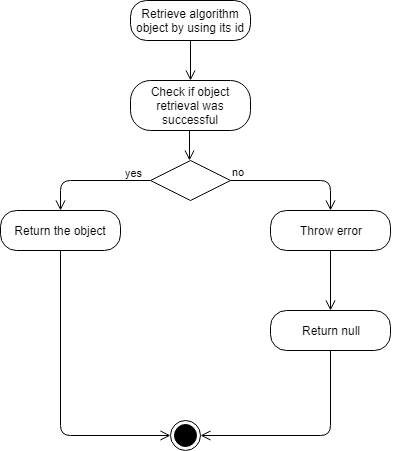
\includegraphics[width=\textwidth]{input_unit/images/get_algorithm_activity_diagram.png}
	\begin{center}
	    \small{Figure 2c: Activity diagram for getting an algorithm }
    \end{center}
    
    \subsubsection{Update An Algorithm's Name}
    \par With regards to Experiment and Data sets attributes, as well as other algorithm's attributes,
{ \textit{Mutatis muntandis} the same as regarding an update to an algorithm's name.} \newline \newline
    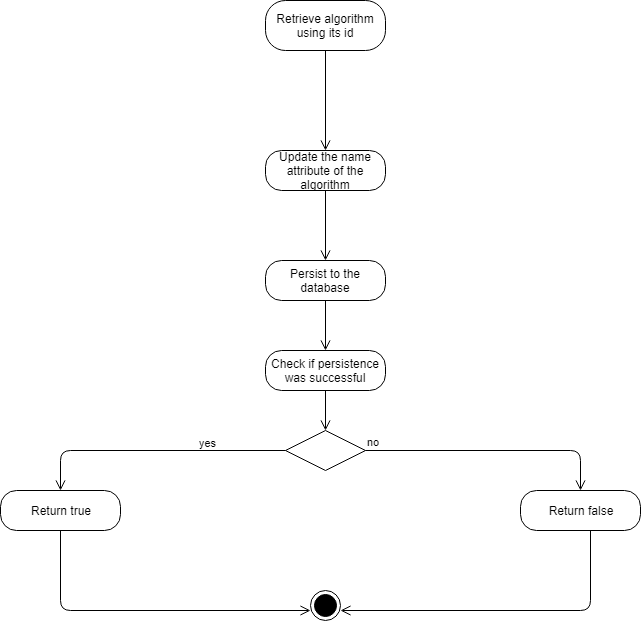
\includegraphics[width=\textwidth]{input_unit/images/update_algorithm_activity_diagram.png}
	\begin{center}
	    \small{Figure 2d: Activity diagram for updating an algorithm's name attribute }
    \end{center}


\subsection{Sequence diagram}
    %\includegraphics[width=\textwidth]{}
	\begin{center}
	    \small{Figure 3: Sequence diagram for Input Unit}
    \end{center}

\subsection{State diagram}
    %\includegraphics[width=\textwidth]{}
	\begin{center}
	    \small{Figure 4: State diagram for Input Unit}
    \end{center}

\subsection{Use Case diagram}
   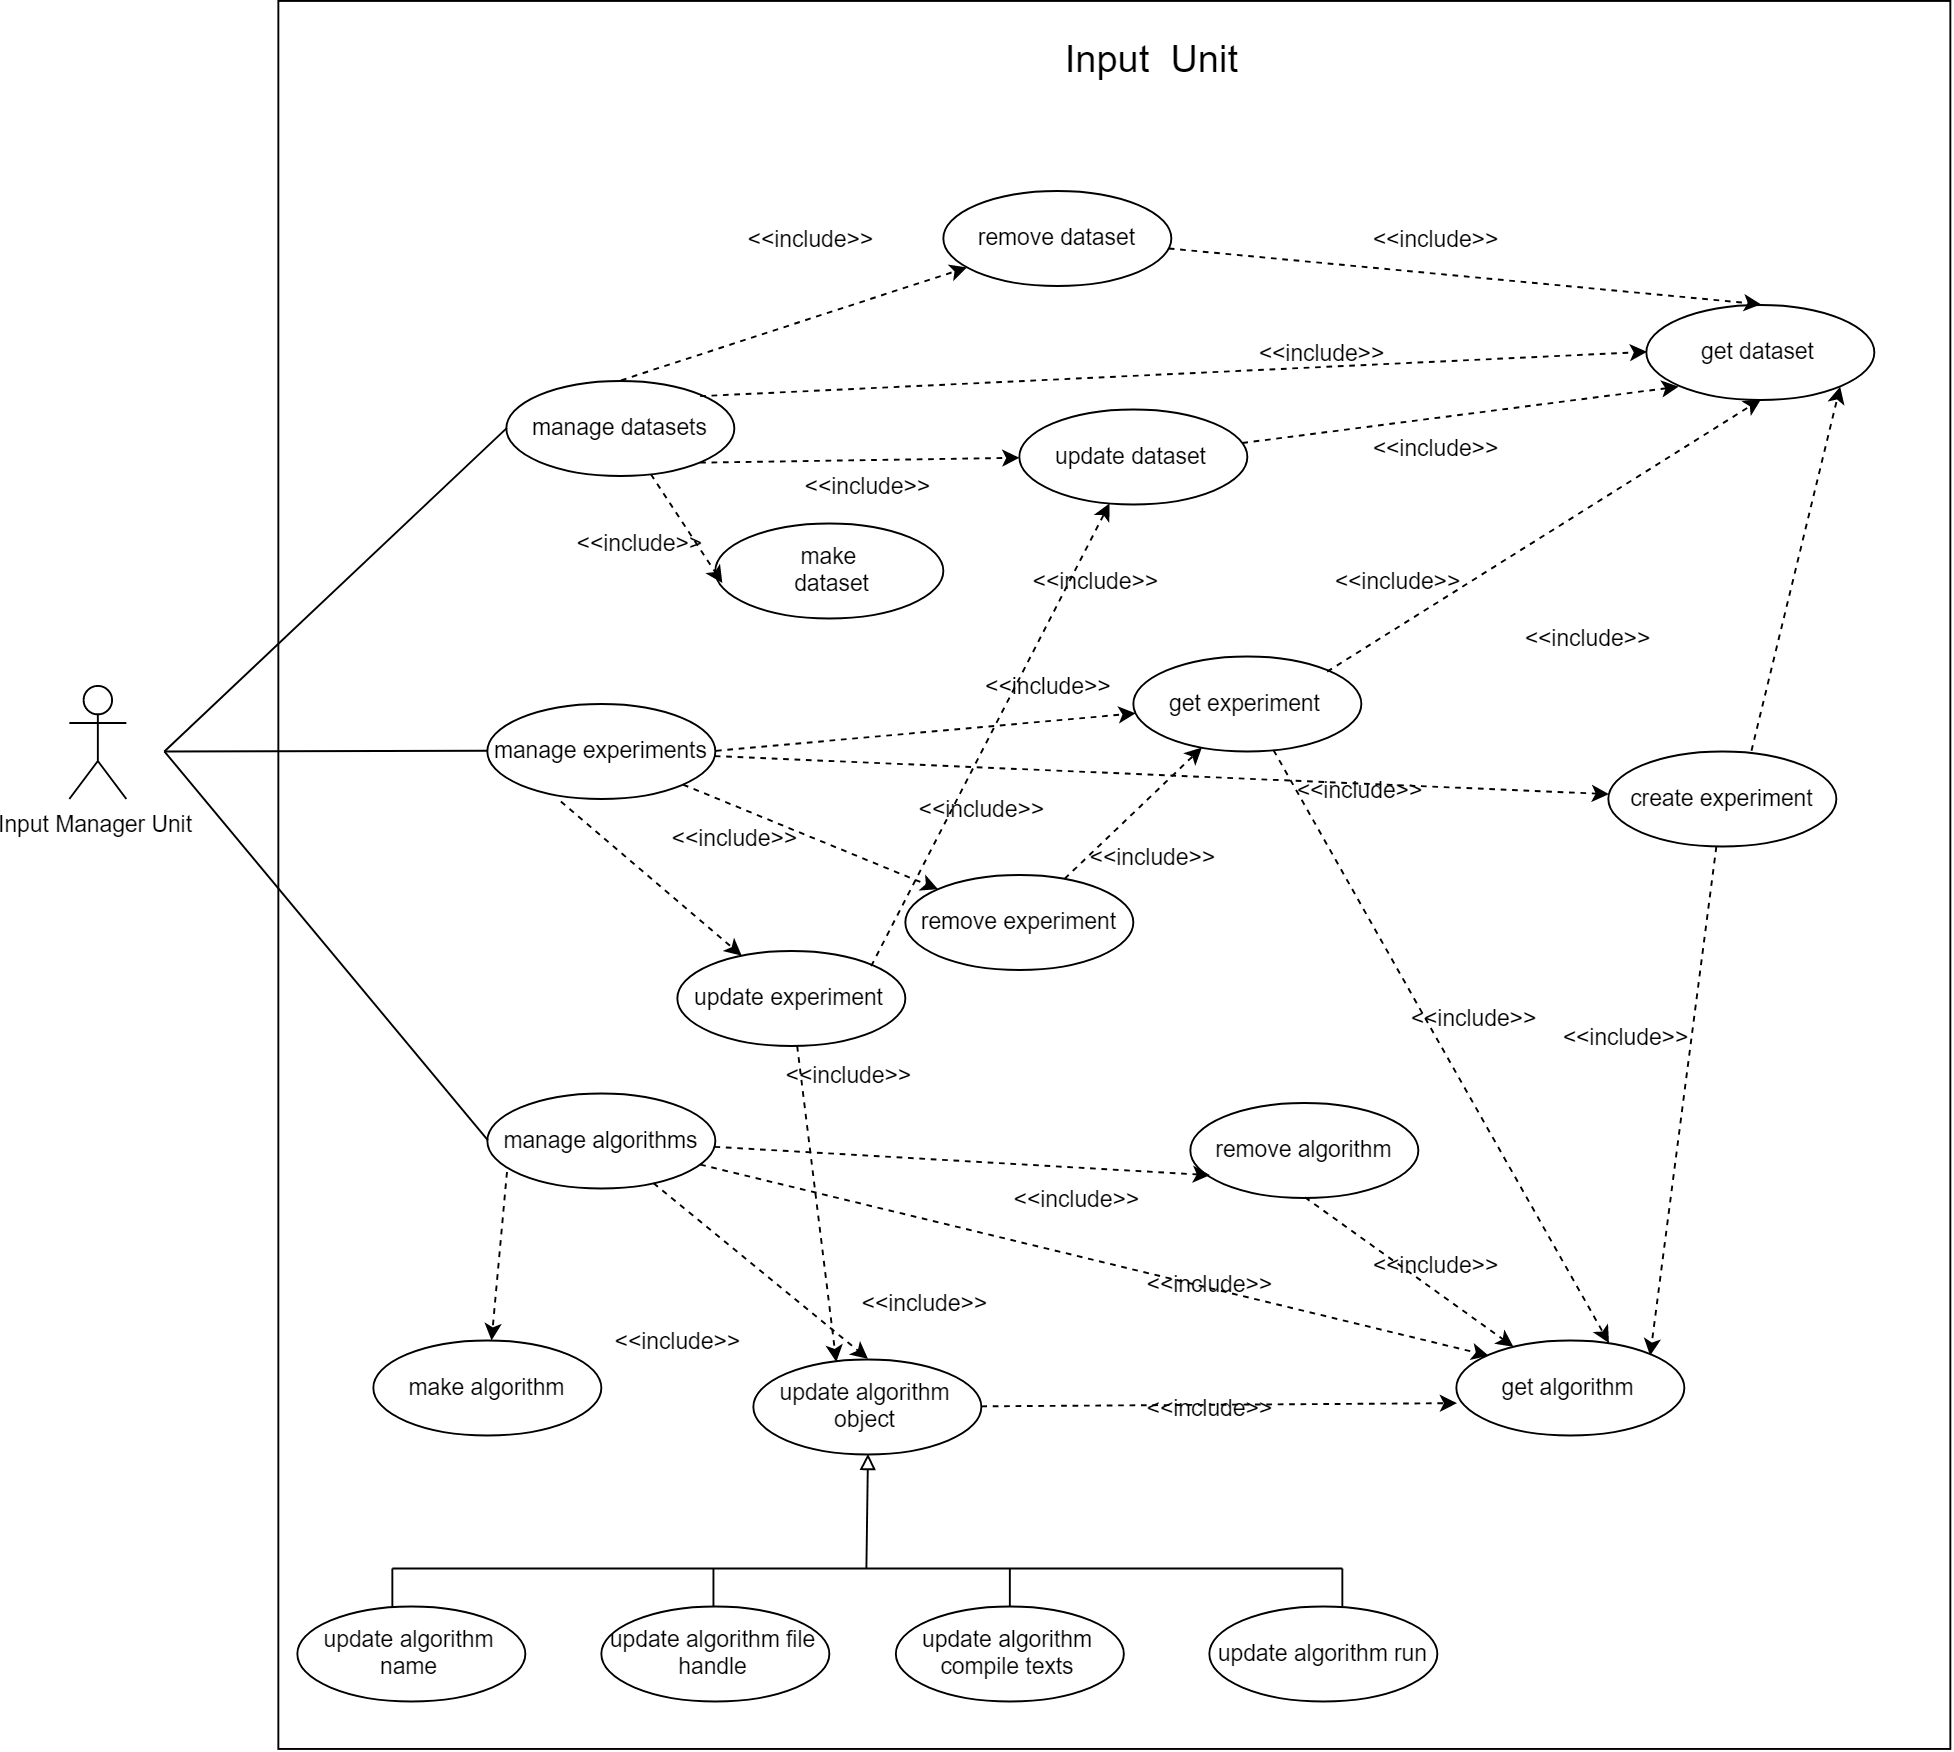
\includegraphics[width=\textwidth]{input_unit/images/input_unit_use_case.png}
    \begin{center}
    	\small{Figure 5: Use case diagram for Input Unit}
    \end{center}